\section{Results}\locallabel{sec:results}
While our initial motivation for this study was to look at the effect of the
feedback delay, the data we collected allowed us to provide answers to
additional questions that have been asked by other researchers. In some cases,
our results confirm those of other researchers, and in others contradict their
previous results. In particular, we compare our results to those of
\spacco{}~\cite{Spacco:2013:TIP:2462476.2465594}. Where our results differ, we
draw conclusions using information from both result sets.

In this section we present the results obtained from an analysis of the 20,777
submissions collected from six classes. We seek to answer the following
questions:

\begin{itemize}
\item Section~\localref{sec:early}: Does Starting Early Help?
\item Section~\localref{sec:time}: Does Time Pressure Affect Behavior?
\item Section~\localref{sec:efficiency}: Does Time Pressure Affect Efficiency?
\item Section~\localref{sec:deadline}: Why Do Students Submit Well After an
  Assignment's Deadline?
\item Section~\localref{sec:sub_impact}: Does Delaying Feedback Impact Student
  Submission Behavior?
\item Section~\localref{sec:session}: Does Delaying Feedback Impact Student
  Work Sessions?
\end{itemize}

\subsection{Does Starting Early Help?}
\locallabel{sec:early}

\begin{figure}[!t]
\centering 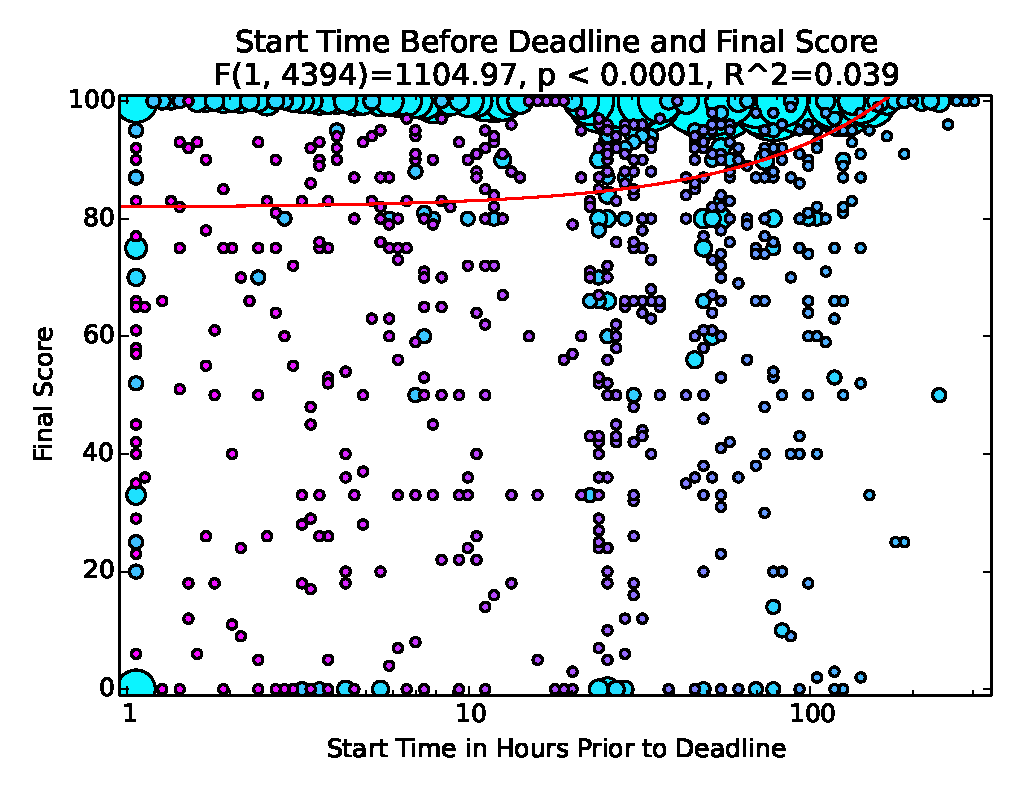
\includegraphics[width=3.3in]{graphs/Start_Time_Before_Deadline_and_Final_Score.eps}
\caption{Compares the number of hours the students started the respective
  assignment prior to the deadline and the final score they received. Both the
  size and color of each circle correspond to the number of groups represented
  at that position. The circles are plotted such that smaller circles are
  strictly in front of larger circles.}
\locallabel{fig:relative_start_time}
\end{figure}

\begin{figure}[!t]
\centering 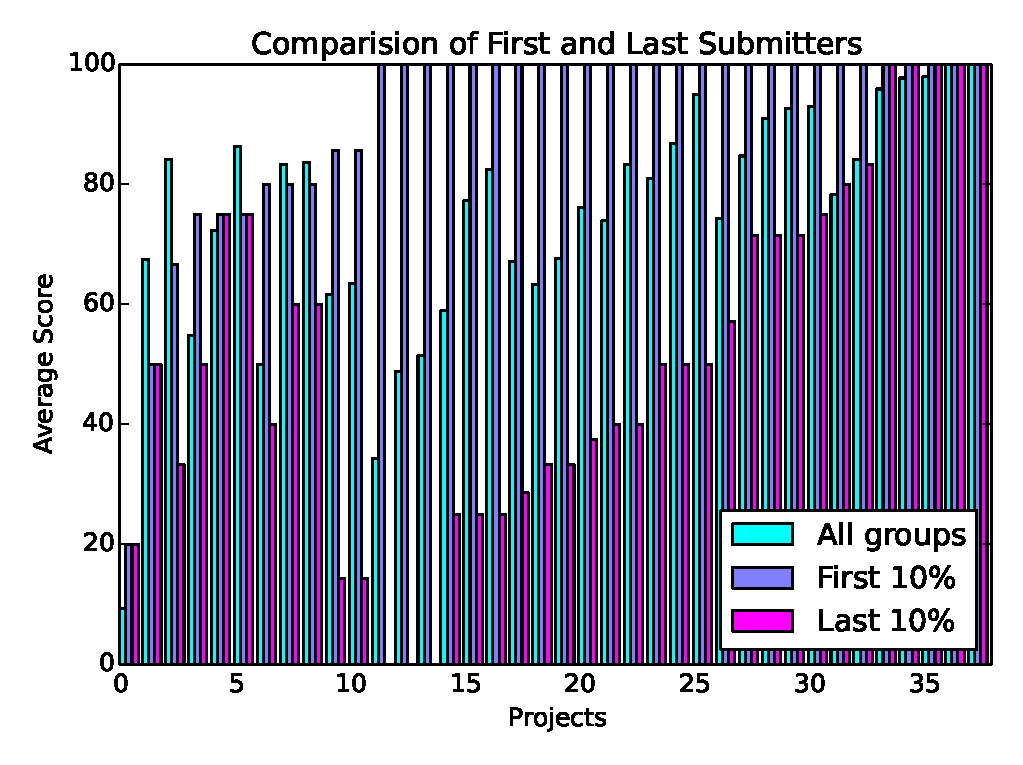
\includegraphics[width=3.3in]{graphs/Comparision_of_First_and_Last_Submitters.eps}
\caption{Compares the average final score of the first 10\% of groups to submit
  to the average and to the last 10\% of groups to submit by project. On
  twenty-seven of the thirty-eight projects the first 10\% of groups had
  perfect scores.}
\locallabel{fig:percent_score}
\end{figure}

Most educators encourage their students to start early on
assignments. Intuitively, starting early gives students more time to receive
feedback and improve the work they submit by the deadline. With a real-time
feedback system, an earlier start provides even more opportunities for feedback
as there are no external human dependencies. Prior work in the field has shown
that such a correlation does in fact
exist~\cite{Spacco:2013:TIP:2462476.2465594,
  Edwards:2009:CEI:1584322.1584325}. We sought to verify that our results were
consistent.

Figure~\localref{fig:relative_start_time} plots the number of hours before an
assignment is due of a group's first submission against the final score the
group receives. Our data statistically significantly correlate earlier
assignment start times with higher scores. While it may seem odd that groups
can receive 100\% on an assignment having started only an hour or less prior to
the deadline, this result is merely an artifact of our active data
collection. Our data collection methodology only provides a lower bound to how
long prior to the deadline a group began working. We verified that small number
of groups distributed uniformly across assignments would make their first
submission in the last hour. This behavior indicates that the groups worked
mostly on their own without using the system in order to receive feedback.

While Figure~\localref{fig:relative_start_time} shows a correlation with start
time and final score, we can break down relative start times even further to a
per-assignment basis. Figure~\localref{fig:percent_score} compares the average
score of the first 10\% of groups to make a submission on an assignment, with
that of all groups, and the last 10\% of groups to make their first
submission. The assignments are sorted according to the first 10\% value, and
then the last 10\% value. Assignments with fewer than 30 groups are excluded so
that at least 3 groups make up each of the 10\% categories. Of the thirty-seven
assignments that meet the criteria, the first 10\% of groups all received 100\%
in twenty-six, with only five where the last 10\% also received 100\%. In the
other twenty-one, the last 10\% scored significantly worse.

In the cases where the first 10\% of groups did not receive 100\% there are a
few outliers where the average is higher than the first 10\% of students to
submit. Of those five cases, all of them were lab assignments in which there
were multiple lab periods. It is likely that a subset of the first 10\% groups
are a group from one of the earlier labs who made an early submission as
directed, but didn't necessarily intentionally start earlier on the assignment.

\subsection{Does Time Pressure Affect Behavior?}
\locallabel{sec:time}

\begin{figure}[!t]
\centering 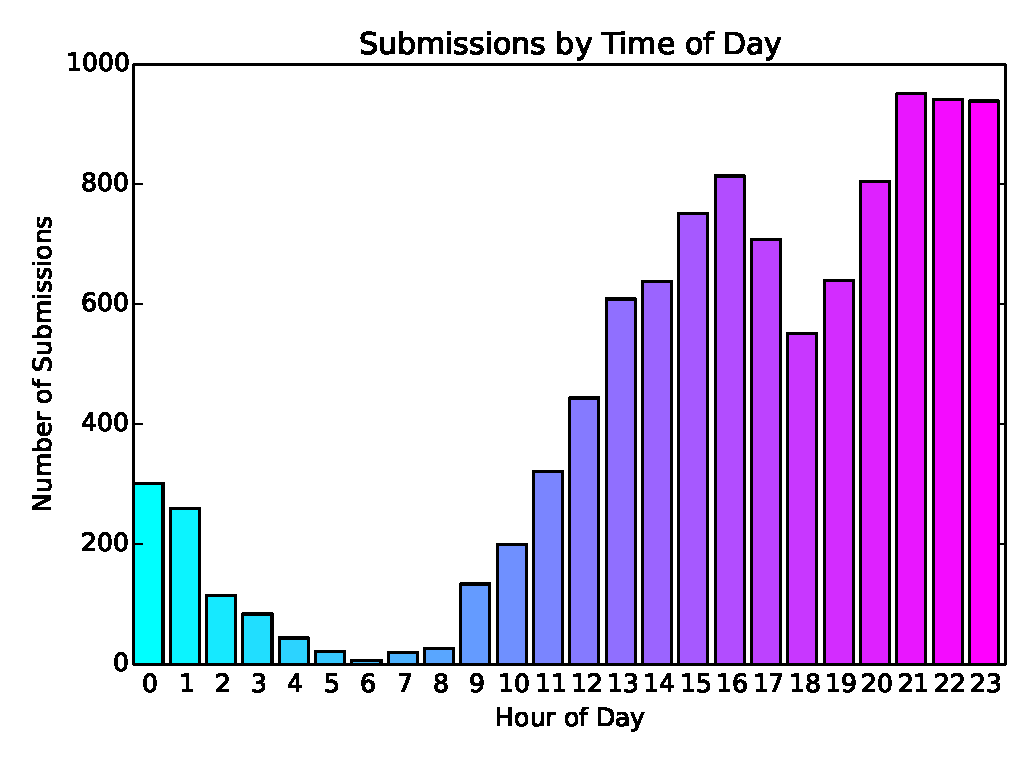
\includegraphics[width=3.3in]{graphs/Submissions_by_Time_of_Day.eps}
\caption{The time of day submissions were made excluding submissions within a
  day of the deadline. Note the \PM{4} peak and the larger peak starting at
  \PM{9} lasting through midnight.}
\locallabel{fig:by_time_far}
\end{figure}

\begin{figure}[!t]
\centering 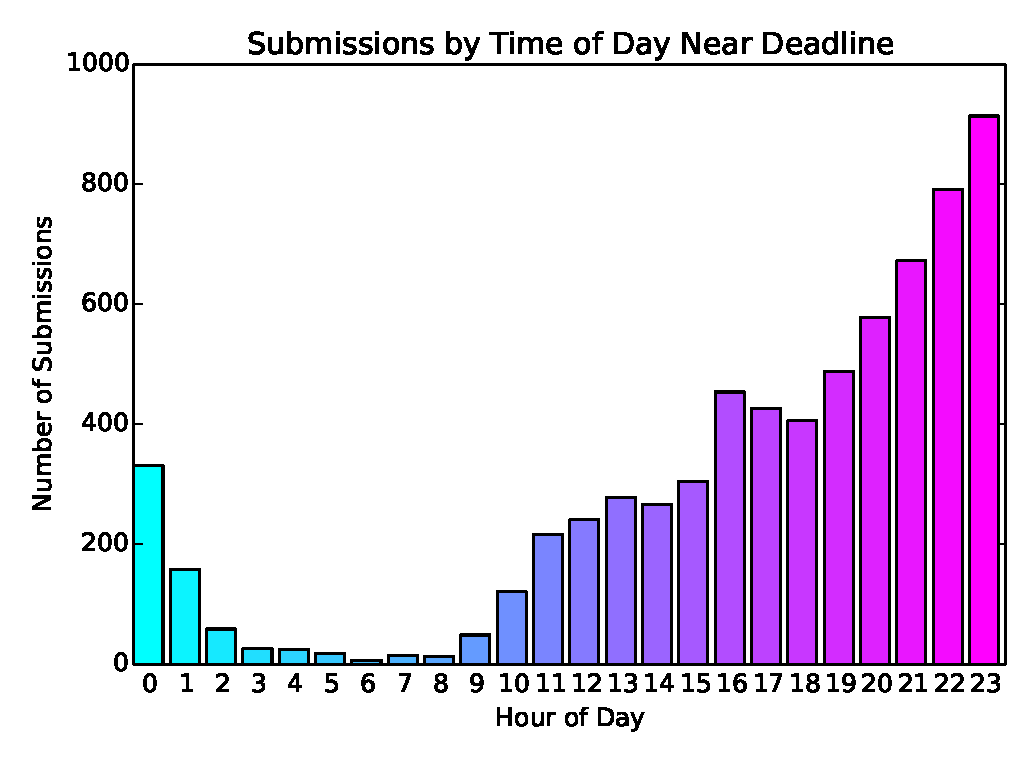
\includegraphics[width=3.3in]{graphs/Submissions_by_Time_of_Day_Near_Deadline.eps}
\caption{The time of day submissions were made including only submissions
  within a day of the deadline. The \PM{11} peak corresponds to the hour prior
  to the deadline for most assignments.}
\locallabel{fig:by_time_near}
\end{figure}

Motivated by the work of \spacco{}, we wanted to see if our active submission
real-time feedback system collected similar student behavior. \spacco{}
discovered their students produced the most work in days prior to the deadline
at \PM{4}, significantly dropping at \PM{6} and remaining nearly consistent
until \AM{1}. Although all of their assignment deadlines were at \PM{6}, they
attributed the peak in work between \PM{4} and \PM{6} as the time that students
preferred to work and thus suggested that ``setting the deadline a couple of
hours later might allow students to work at their preferred time without the
added pressure of an impending deadline''
~\cite{Spacco:2013:TIP:2462476.2465594}. Our results indicate otherwise.

Figure~\localref{fig:by_time_far} depicts the number of submissions made at
each time of day for submissions made more than a day from the deadline. We
observe a steady increase in the number of submissions beginning at \AM{9} and
peaking at \PM{4}. This peak is followed by decrease through \PM{6}. Up to this
point, our results are nearly identical to that of \spacco{}. However, rather
than observing a consistent amount of work for the remainder of the night, we
observe an even larger increase in work until \PM{9} where the amount of work
remains nearly consistent until midnight. Thus, while our students are
productive between \PM{4} and \PM{6}, they are even more productive in the
three hours before midnight. Coincidentally, seventy-one out of seventy-six of
our assignments had a midnight deadline. This observation combined with the
results of \spacco{} leads us to believe that students learn to work most
efficiently in the hours just prior to an expected deadline.

As previously indicated, we excluded submissions from
Figure~\localref{fig:by_time_far} that were made within one day of their
deadline. Our hypothesis was that a more significant majority of the
submissions would be made in the hours just prior to their assignment
deadline. Figure~\localref{fig:by_time_near} confirms that hypothesis. While
there is little change in the figure shape prior to \AM{11}, the there is only
a slight increase in work during the \AM{11} to \PM{3} range. A sharp spike in
submissions occurs at \PM{4} and has a gradual decrease until \PM{6}. This
decrease in submissions occurs in both figures, and we suspect this decrease
corresponds with the time students leave campus, head home, and eat dinner,
prior to resuming work. Finally, we observe a consistent increase in work right
up to midnight, the most common deadline.

It is important to note that this data include an insignificant amount of
error. Prior to the introduction the \emph{group} feature to the submission
system, it was common for multiple members of a group to make independent
submissions to the system, often only submitting the final complete version of
the assignment. We detected and excluded eighty-seven subsequent exact
duplicate submissions (0.4\%). Of these, seventeen (20\%) occurred in the
\PM{11} hour. However, only nine (10\%) occurred in the hour prior to the
deadline. While we detected and excluded subsequent identical submissions, we
do not do the same for nearly-identical submissions because the error they
introduce is insignificant. We come to this conclusion by assuming there are
a similar number of undetected non-exact duplicate submissions and that these
submissions have a similar hour-prior to deadline distribution.

\subsection{Does Time Pressure Affect Efficiency?}
\locallabel{sec:efficiency}

\begin{figure}[!t]
\centering 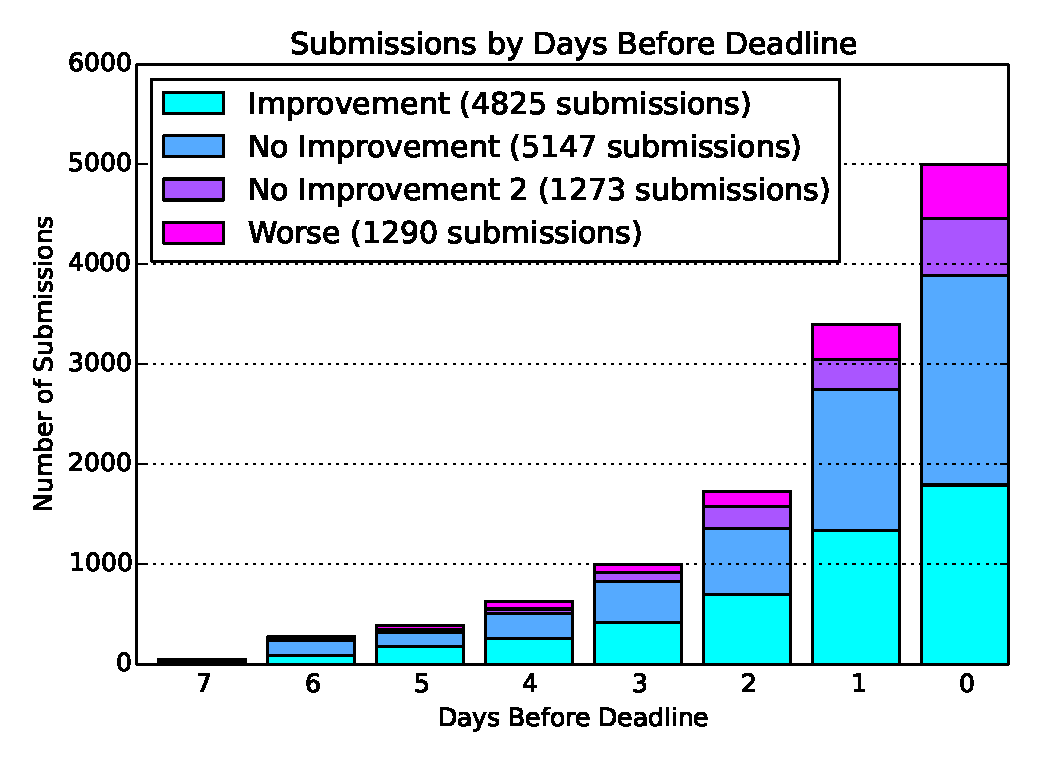
\includegraphics[width=3.3in]{graphs/Submissions_by_Days_Before_Deadline.eps}
\caption{Number of submissions by the number of days prior to the deadline
  grouped by improvement category.  Submissions that improve the group's
  maximum project score is considered \emph{Improvement}, those that tie are
  \emph{No Improvement}. \emph{Worse} submissions are those that result in a
  local minimum, and all submissions between the group's maximum project score
  and the local minimum is labeled \emph{No Improvement 2}.}
\locallabel{fig:days_submissions}
\end{figure}

\begin{figure}[!t]
\centering 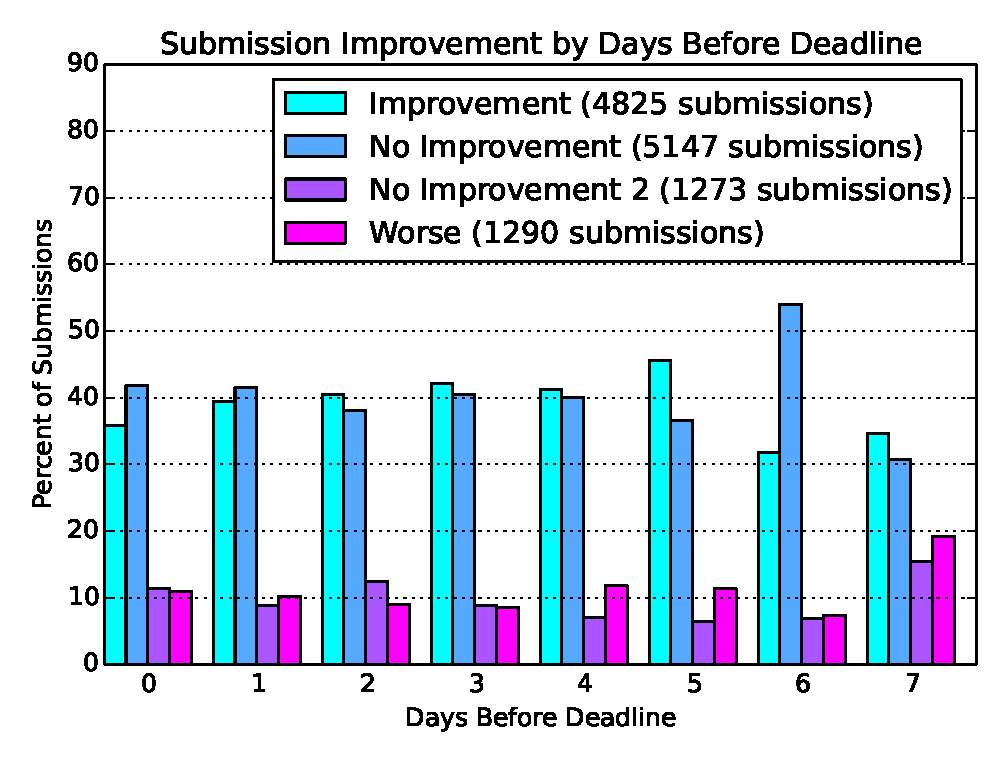
\includegraphics[width=3.3in]{graphs/Submission_Improvement_by_Days_Before_Deadline.eps}
\caption{Percentage of submissions in each improvement category by the number
  of days prior to the deadline.}
\locallabel{fig:days_improvement}
\end{figure}

The previous section described at how submission behavior is altered by an
assignment deadline. In this section we look at the effect of a pending
deadline on submission efficiency. There are a number of ways one could define
efficiency between submissions. One metric is to look at amount of change in
source code between submissions. Another is to look at the change in cyclomatic
complexity between submissions. While each of these metrics may provide
interesting insights into student behavior, we are more interested in
correlations with changes in students' scores between submissions. Thus, we
consider efficiency by looking at improvements or regressions in subsequent
submissions based on the change in score. The score is altered by a submission
passing more or fewer tests. We quantify changes in submission efficiency by
classifying subsequent submissions into one of four categories:

\begin{description}
  \item[Improvement] \hfill \\ The submission increases the group's maximum
    score on the project.
  \item[No Improvement] \hfill \\ The submission has the same score as the
    group's running maximum score.
  \item[No Improvement 2] \hfill \\ The submission's score is less than the
    running maximum score and is not lower than the localized minimum score.
  \item[Worse] \hfill \\ The submission results in a localized minimum
    score. That is, it is the lowest score since the last \emph{Improvement}
    submission.
\end{description}

Figure~\localref{fig:days_submissions} depicts the total number of submissions
made in the days prior to the each submission's respective deadline according
to their respective category. The figure only extends to seven days as the
number of submissions more than seven days prior to the deadline is
insignificant. Our results show that a majority of submissions are made in the
two days prior to the deadline and this observation is consistent with
\spacco{}. In contrast, however, we observe a much higher percentage of \imp{}
submissions when compared to their \emph{positive}
snapshots~\cite{Spacco:2013:TIP:2462476.2465594}.

The likely reason for this discrepancy is the difference between their
passively collected snapshots and our actively collected submissions. Where a
snapshot may not represent a complete unit of work, a submission often does as
groups explicitly make submissions in order to receive feedback. One other
difference is our \imp{} submissions are only submissions that improve upon a
group's maximum score. It is unclear from \spacco{}'s description if a snapshot
that improves the score of a \emph{negative} snapshot is considered
\emph{positive} even its score does not improve the student's maximum score. If
this is the case, then the number of \emph{positive} snapshots is inflated in
their results when compared to ours.

Regardless, we think the comparison of efficiency between submissions is more
interesting than comparison between snapshots as there are still a significant
number of submissions that are not
\imp{}. Figure~\localref{fig:days_improvement} shows the relative percent of
submissions in each category by the number of days prior to the
deadline. Overall, the difference in efficiency is insignificant with respect
to the number of days prior to the deadline. While our deadlines were
distributed such that 24\% and 25\% of submissions were made for assignments
with a Monday and Friday deadline respectively, there was no difference in
efficiency with respect to the day of week a submission was made on.

An analysis of the hour of day of each submission both generally and
specifically for submissions on the day of their deadline also produced no
significant changes in efficiency. Thus, these results convince us that time
pressure does not affect efficiency. Nevertheless, they provide useful insight
to overall efficiency and any changes to the system or student behavior that
increases efficiency should be further studied.

\subsection{Why Do Students Submit Well After an Assignment's Deadline?}
\locallabel{sec:deadline}

\begin{figure}[!t]
\centering 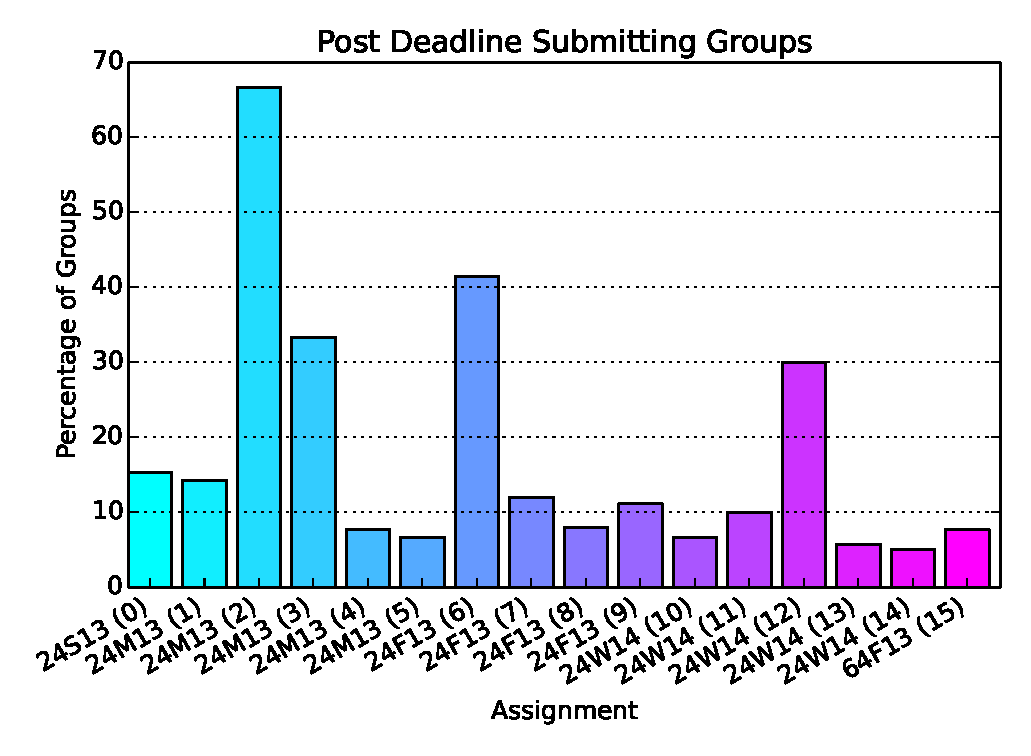
\includegraphics[width=3.3in]{graphs/Post_Deadline_Submitting_Groups.eps}
\caption{The percentage of groups who submit more than two days following an
  assignment's deadline.}
\locallabel{fig:late}
\end{figure}

An interesting aspect of real-time feedback systems that prior work has not
touched upon is student usage of such systems beyond the assignment deadline in
order to make improvements and verify the correctness of those
improvements. These systems provide inherently provide this functionality and
some students take advantage of it.

Figure~\localref{fig:late} shows the percentage of groups by project who
submitted more than two days after the respective project deadline. Of the
seventy-six projects, only sixteen are shown in the figure. Five assignments
were excluded for representing fewer than ten groups. Such assignments were
often the first assignment of the quarter for which we had only received a
portion of the consent forms. Twenty-nine assignments had zero post-deadline
submitting groups thus are not shown. Additionally, twenty-six assignments had
between 1\% and 4\% (average 2.4\%) of groups with post deadline
submissions. These assignments are excluded from the figure for space purposes.

Two days was chosen as the cutoff point because by this time all students were
beyond any late-credit that may have been offered across all projects. Except
where otherwise noted, submissions occurring after this two-day period provide
the student with no direct grade-benefits. The projects are grouped by class
along the x-axis.

Five of the of the assignments in Figure~\localref{fig:late} are from
\cm[24]{13}, which had only seventeen consenting students whereas the next
smallest class, \cs[64]{14}, had forty-eight consenting students. \cm[24]{13}'s
small class size is significant as a higher percentage of the students were
able to receive assistance in office hours from both the teaching assistant and
the instructor.

Additionally, five of the assignments are from \cw[24]{14}. In this class, half
of the groups submitting post deadline did so for more than one assignment. We
discovered the majority of these post deadline submissions to occur just prior
to one of the course examinations. This discovery suggests that a number of
students utilized the real-time feedback system as an aid for exam
studying. Messages on the course discussion group confirmed students utilized
the submission system to improve upon previous course assignments as a form of
exam preparation.

Overall, four of the assignments, \emph{2}, \emph{3}, \emph{6}, and \emph{12},
stand out from the remainder. The first two, \emph{2}, and \emph{3}, were
assignments that subsequent assignments depended on. Thus, as reported by the
instructor, many students sought help during office hours to correct any issues
prior to moving on to the following assignment. The instructor reported that
the real-time feedback system was invaluable during office hours to efficiently
verify correctness of modifications to students' programs without exposing the
test cases, nor requiring the instructor to manually obtain and test the
students' in-progress work. Assignment \emph{6} presented students with the
opportunity to make-up missed points after the deadline, thus, not surprisingly
explaining its spike in post deadline submissions. Finally, assignment
\emph{12} both had a number of students revisit prior to a class exam, and was
a dependency of a subsequent assignment.

Thus these results show that there are three primary reasons why students
continue to work on assignments well after the deadline:

\begin{itemize}
\item Intuitively, the most prominent reason we observed is for make up
  credit. While abusing this functionality may result in students not taking
  the initial deadline seriously, with the support of a real-time feedback
  system, very little human resources are required.
\item The second most prominent reason we observed is due to inter-assignment
  dependency. When one assignment depends on the work of a former assignment a
  number of students found it useful to be able to verify correctness of
  improvements made to the dependent part of code.
\item Finally, we observed a small number of students who made improvements to
  past assignments as part of studying for their examinations.
\end{itemize}

Overall we consider any submissions made after the deadline to be a success of
the real-time feedback system. Without lowering the barriers to additional
feedback, these students may have not made any effort to improve upon their
past assignments.

\subsection{Does Delaying Feedback Impact Student Submission Behavior?}
\locallabel{sec:sub_impact}

\begin{figure}[!t]
\centering 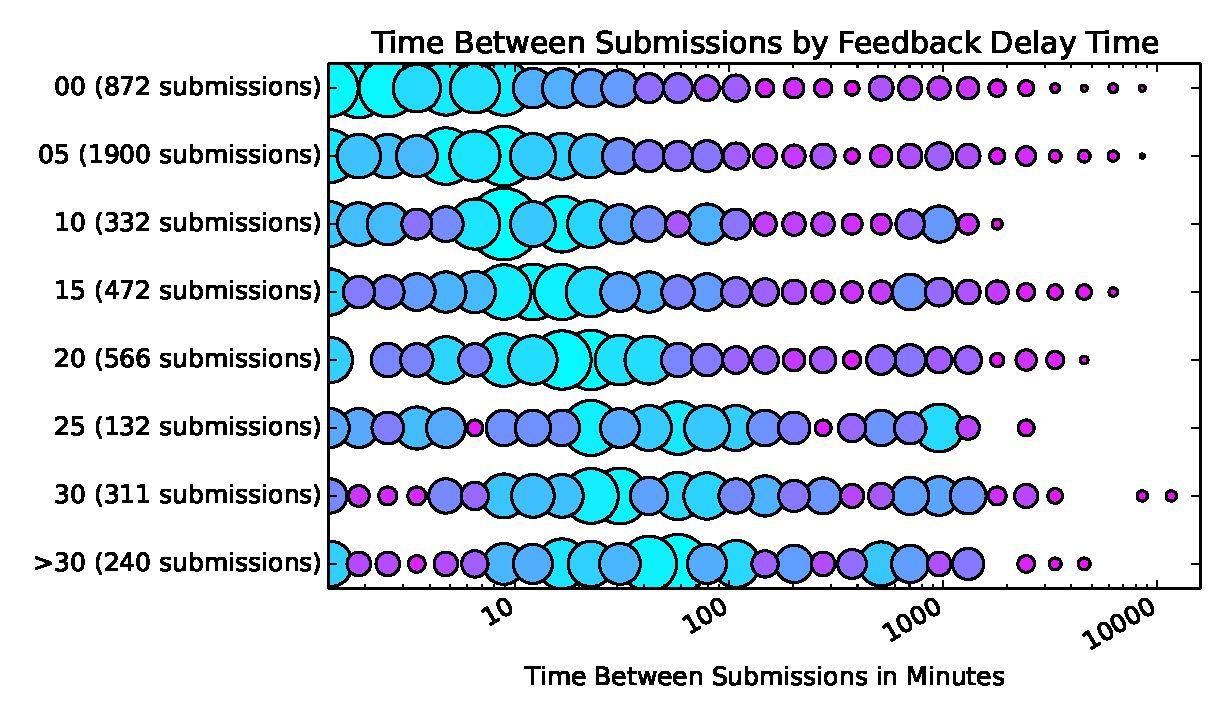
\includegraphics[width=3.3in]{graphs/Time_Between_Submissions_by_Feedback_Delay_Time.eps}
\caption{Plots the time between submissions grouped by assignment feedback
  delay. Note the shift to a longer time between submissions in largest
  grouping as the delay increases.}
\locallabel{fig:delta_delay}
\end{figure}

\begin{figure}[!t]
\centering 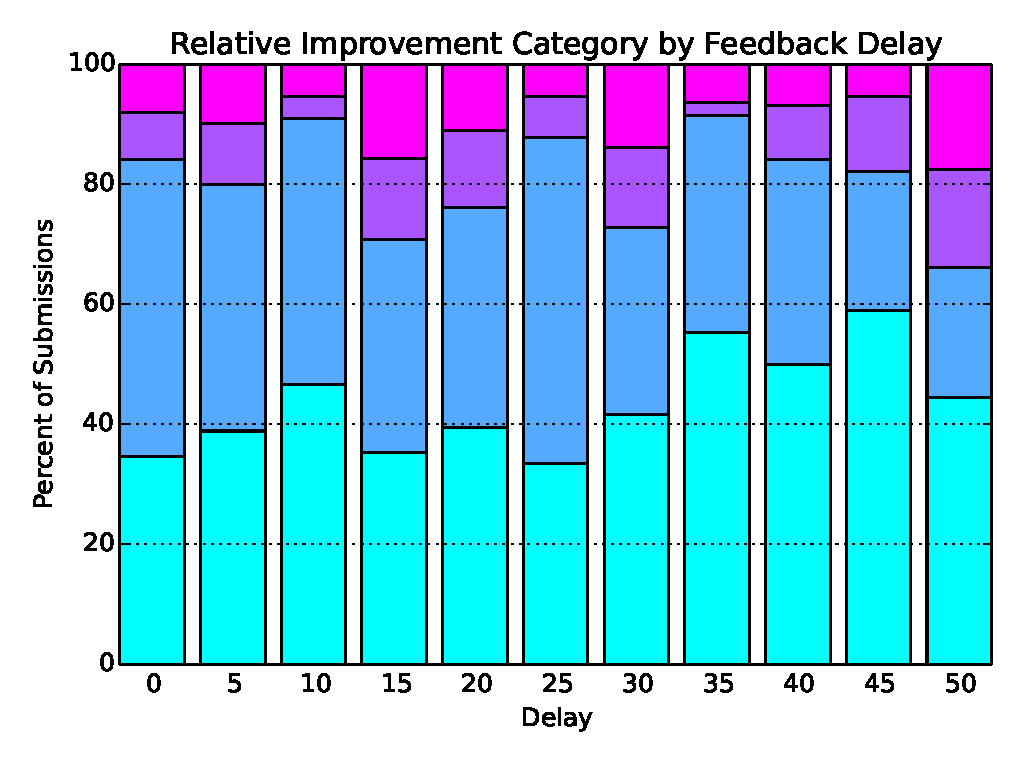
\includegraphics[width=3.3in]{graphs/Relative_Improvement_Category_by_Feedback_Delay.eps}
\caption{Plots the time between submissions grouped by assignment feedback
  delay. Note the shift to a longer time between submissions in largest
  grouping as the delay increases. Refer to
  Figure~\localref{fig:days_improvement} for the legend.}
\locallabel{fig:delta_efficiency}
\end{figure}

\begin{figure}[!t]
\centering 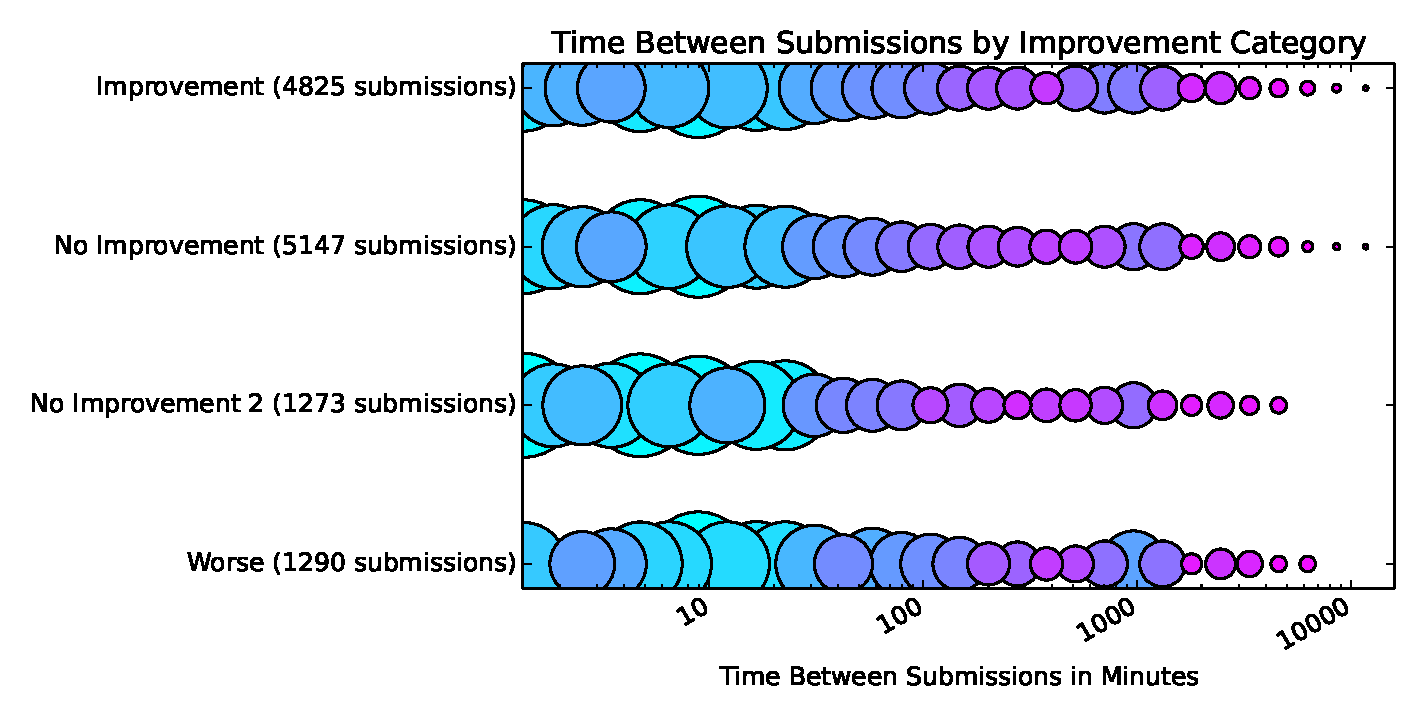
\includegraphics[width=3.3in]{graphs/Time_Between_Submissions_by_Improvement_Category.eps}
\caption{Plots the time between submissions by their improvement category.}
\locallabel{fig:delta_category}
\end{figure}

As indicated in section~\localref{sec:delay}, we sought to measure the impact
that altering the feedback delay has on student behavior. In this section, we
present the those results. We first look at the impact of the delay on the time
between submissions. Figure~\localref{fig:delta_delay} plots the time between
subsequent submissions grouped by each of the assignment feedback delay
times. Note the y-axis is shown in a log-scale and the size and color of the
circle represent the number of submission gaps represented by the individual
circle. The figure clearly shows an increasing amount of time between
submissions for the largest grouping of gaps as the delay increases.

Figure~\localref{fig:delta_efficiency} shows the relative efficiency of
submissions grouped by the feedback delay. The results appear to indicate that
there is a significant improvement in efficiency with delays of thirty minutes
or more. Using Student's t-test, we compared the percent of \imp{} submissions
for each feedback delay under thirty minutes, to those of each feedback delay
thirty minutes or longer. The difference was statistically significant with
P=0.0095.

For comparison, Figure~\localref{fig:delta_category} depicts the time between
submissions for each of the improvement categories. The aggregate results from
the figure indicate that the most common time between a group's submissions is
approximately ten minutes. Furthermore, there is a consistent spike in time
between submissions just prior to the 1000 minute mark. Overall, there is not a
significant difference in time between submissions with respect to improvement
category. However, the shape of the individual scatter lines provide two
insights:

\begin{itemize}
\item Relatively the most \noii{} submissions occur in the first few seconds as
  indicated by the size and color of its first circle compared to the other
  categories. Recall that \noii{} submissions occur in the period after a
  \worse{} submission and prior to a \imp{} submission. The short period of
  time between these submissions and their corresponding former submissions is
  too small for students to have understood any feedback they may have received
  and suggests the students did not independently test whatever changes they
  made prior to resubmission.
\item Interestingly, with respect to \worse{} submissions, the spike around the
  1000 minute mark, is the most significant compared to other categories. This
  data suggest that long breaks have an initially negative impact on assignment
  progress.
\end{itemize}

These results confirm that changes in the feedback delay has an impact on
student submission behavior. In general, as the delay increases students wait
longer to submit, and when comparing delays of less than thirty minutes to
those of thirty or more minutes, the students are more likely to improve upon
their previous score.

\subsection{Does Delaying Feedback Impact Student Work Sessions?}
\locallabel{sec:session} Section~\localref{sec:sub_impact} showed that a delay
in feedback has an impact on both the time between submissions and the
likeliness for submissions to improve upon the previous submission. In this
section we attempt to group submissions into a work session. This grouping
allows us to both look at the affect of the feedback delay on work session, and
to compare our work session results to prior work. We define a work session
similarly to \spacco{}. Specifically, we define a work session as a collection
of submissions by the same group for the same assignment where in which there
is no gap between any two of these submissions larger than some window size.

\subsubsection{Determining an Appropriate Window Size}
\locallabel{sec:window}

\begin{figure}[!t]
\centering 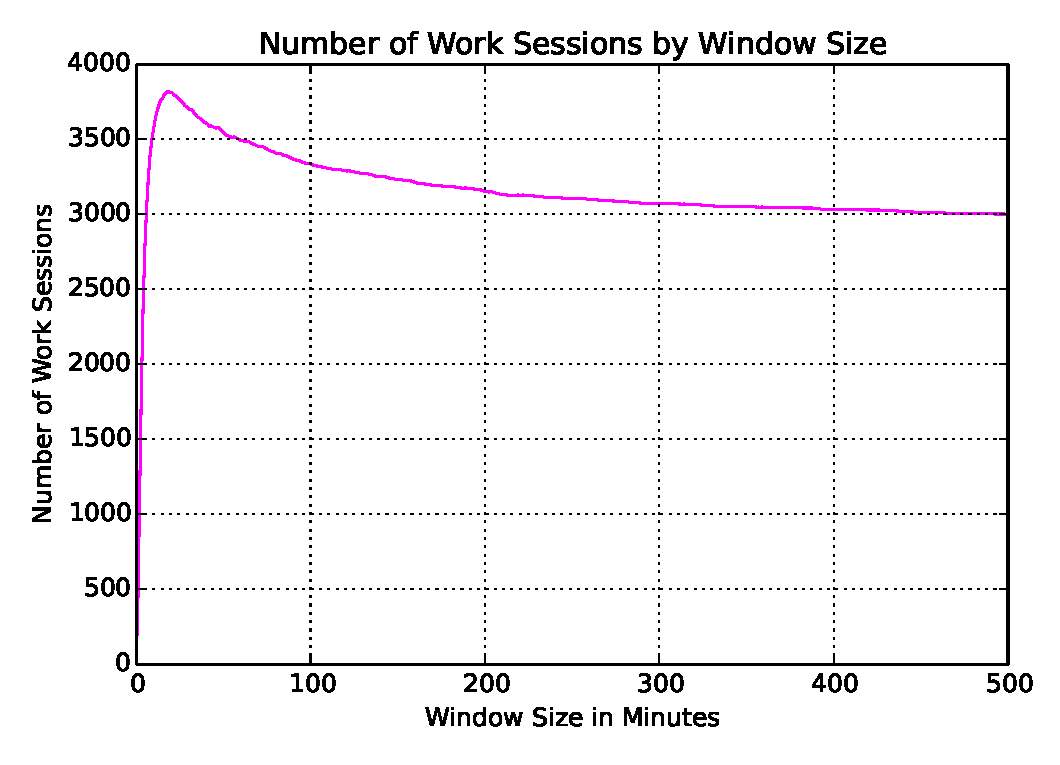
\includegraphics[width=3.3in]{graphs/Number_of_Work_Sessions_by_Window_Size.eps}
\caption{Plots the number of work sessions as the window size increases.}
\locallabel{fig:work_sessions}
\end{figure}

\begin{figure}[!t]
\centering 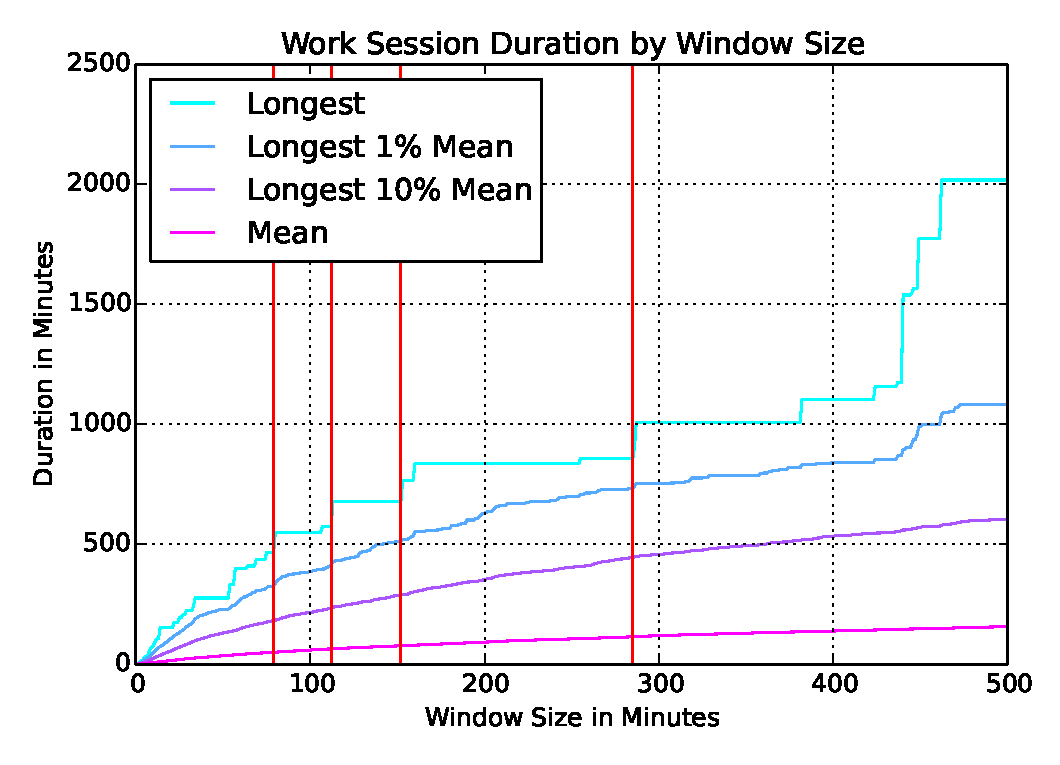
\includegraphics[width=3.3in]{graphs/Work_Session_Duration_by_Window_Size.eps}
\caption{Shows the change in work session duration as the window size
  changes. The red vertical lines indicate points of interest due to
  significant changes in the longest duration work session. The red lines occur
  at window sizes 79, 112, 152, and 285.}
\locallabel{fig:window_size}
\end{figure}

We investigate the ideal window size for which to discover work
sessions. \spacco{} arbitrarily chose a window size of twenty
minutes~\cite{Spacco:2013:TIP:2462476.2465594}. While this window size may have
been appropriate for their data set where snapshots were collected passively
upon changes, it is not appropriate for our data set due to the fact that
students actively submitted only when they desired feedback. Furthermore, we
have assignments with a feedback delay of fifty minutes, where students
regularly make no more than one submission in any fifty minute
period. Therefore, the window size we select to group submissions into work
sessions must be at least fifty minutes in length.

There are two forms of error that we must mitigate when selecting a window
size. The first is error in distinguishing between work and non-work time
within the window size. Intuitively, this error is reduced by minimizing the
window size due to the fact that any non-work periods longer than the window
size will not be included as part of the work session. The second is error in
classifying the time between two submissions as part of the previous work
session or not. For instance, if we select the window size as sixty minutes,
then this error corresponds to the number of subsequent submissions that occur
over sixty minutes which represent work time. While we can measure the number
of subsequent submissions over a given window size, we cannot measure either
error due to a lack of information as to when students are actually working. We
accept these errors, and assume that it equally effects working sessions
independent of the feedback delay time.

Rather than arbitrarily choosing a value, we attempt to select an idea window
size based on features of our data. We use the maximum session length as a
heuristic for limiting the window size as it is unlikely that more than a
handful of all sessions are longer than eight hours plus some additional time
to account for error due to breaks during one or more
windows. Figure~\localref{fig:work_sessions} shows the effect of increasing the
window size on the number of work sessions created. This figure shows that for
our data the maximum number of work sessions occurs with a window size of
approximately twenty minutes, after which the number of work sessions gradually
decreases. This decrease indicates that as the window size grows, more work
sessions are merged together than the number of new work sessions created by
grouping two independent submissions together. Aside from the twenty minute
peak, there are no other points of interest in this figure.

Figure~\localref{fig:window_size} plots a number of lines corresponding to
various work session lengths as the window size increases. The four
non-vertical lines correspond to:

\begin{itemize}
\item the duration of the single longest work session
\item the mean duration of the top 1\% of work sessions sorted by length
\item the mean duration of the top 10\% of work sessions sorted by length
\item the mean duration of all work sessions
\end{itemize}

Of these four lines, we find only the duration of the single longest work
session to be of interest as there are a number of distinct window sizes that
result in increasing the longest duration. The red vertical lines on the figure
highlight the window sizes of interest, that is, they are the window sizes just
prior to a significant increase in maximum work session length. We excluded
consideration of points of interest at larger window sizes as it is infeasible
for 10\% of all work sessions to be over eight hours in length. Additionally we
exclude the point of interest that occurs just after fifty minutes due to its
proximity with our longest feedback delay.

We select the left-most point of interest, seventy-nine minutes, as the window
size we use in the remainder of the results section. Note, however, that where
statistical significance is concerned, we verified that each highlighted window
size in Figure~\localref{fig:window_size} produces consistent results with
those produced using the seventy-nine minute window size. This comparison shows
that our analysis is unaffected by the specific choice of window size from
those we highlighted.

\subsubsection{Properties of Work Session Lengths}

\begin{figure}[!t]
\centering 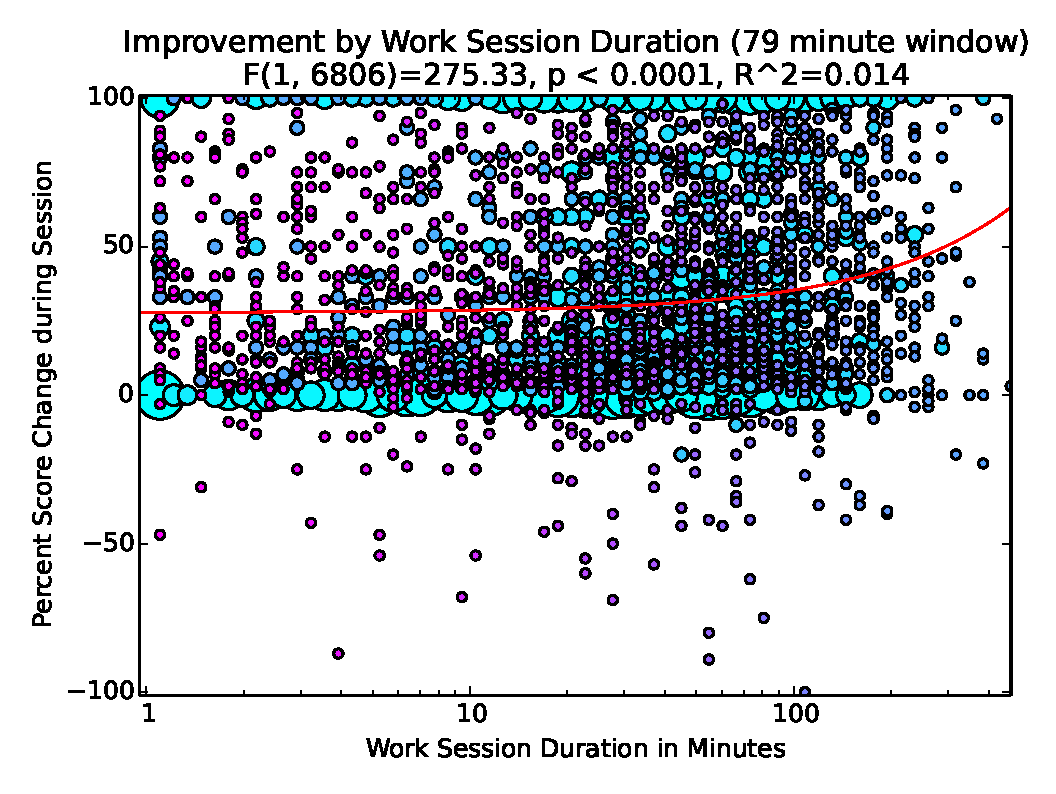
\includegraphics[width=3.3in]{graphs/Improvement_by_Work_Session_Duration_(79_minute_window).eps}
\caption{Depicts a positive correlation between work session duration and
  percent score change. The results are statistically significant according to
  an F-test.}
\locallabel{fig:session_improvement}
\end{figure}

\begin{figure}[!t]
\centering 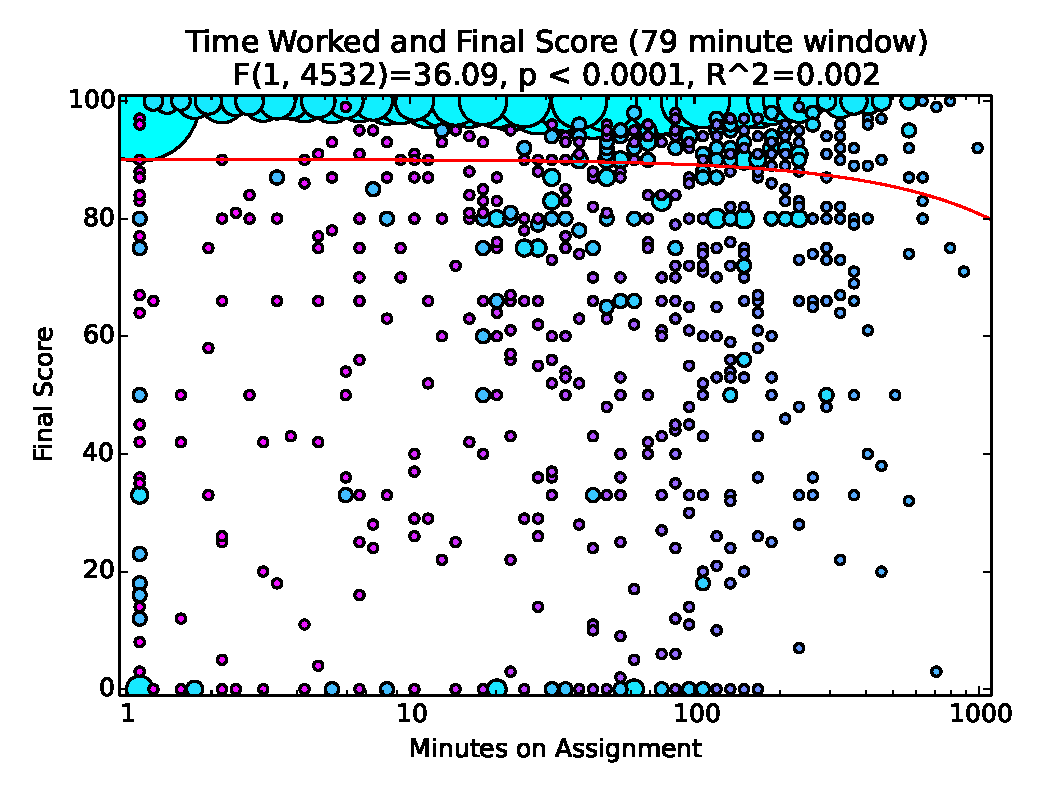
\includegraphics[width=3.3in]{graphs/Time_Worked_and_Final_Score_(79_minute_window).eps}
\caption{Depicts a negative correlation between the minutes spent on an
  assignment and the final score. The results are statistically significant
  according to an F-test.}
\locallabel{fig:time_score}
\end{figure}

Before considering the impact the feedback delay has on work session, we first
compare some general properties of our work sessions to that of the work
sessions discovered by \spacco{}.

Using our window size, we are able to group submissions into work sessions, and
thus approximate the length of a work session as the time between the first and
last submission in a work session. Rather than looking at the improvement
between individual submissions as we did in
Figure~\localref{fig:delta_category}, Figure~\localref{fig:session_improvement}
plots the percent score change made between the first and last submissions in a
work session against the length of the work session. In this figure circles at
the 0\% change would be considered \noi{}, and a significant majority of
sessions would be considered \imp{} due to the significant imbalance between
the number of sessions that improve the score as compared to those which reduce
the score. The red-line is the trend-line and an F-test of the data confirms
that that there is a statistically significant correlation between the length
of a work session and the percent of score change. Our results are consistent
with those of \spacco{}~\cite{Spacco:2013:TIP:2462476.2465594}.

An approximation of total time spent on an assignment can be made by summing
the length of all the work sessions by group for an
assignment. Figure~\localref{fig:time_score} plots the final score compared to
the total time spent on an assignment. The red-line shows there is a
statistically significant negative trend. This indicates that the longer
students work on an assignment the less likely they are to score well. These
results contradict the results of \spacco{} where they found a statistically
significant positive correlation.

\subsubsection{Impact of Feedback Delay on Work Sessions}
\locallabel{sec:session_impact}

\begin{figure}[!t]
\centering 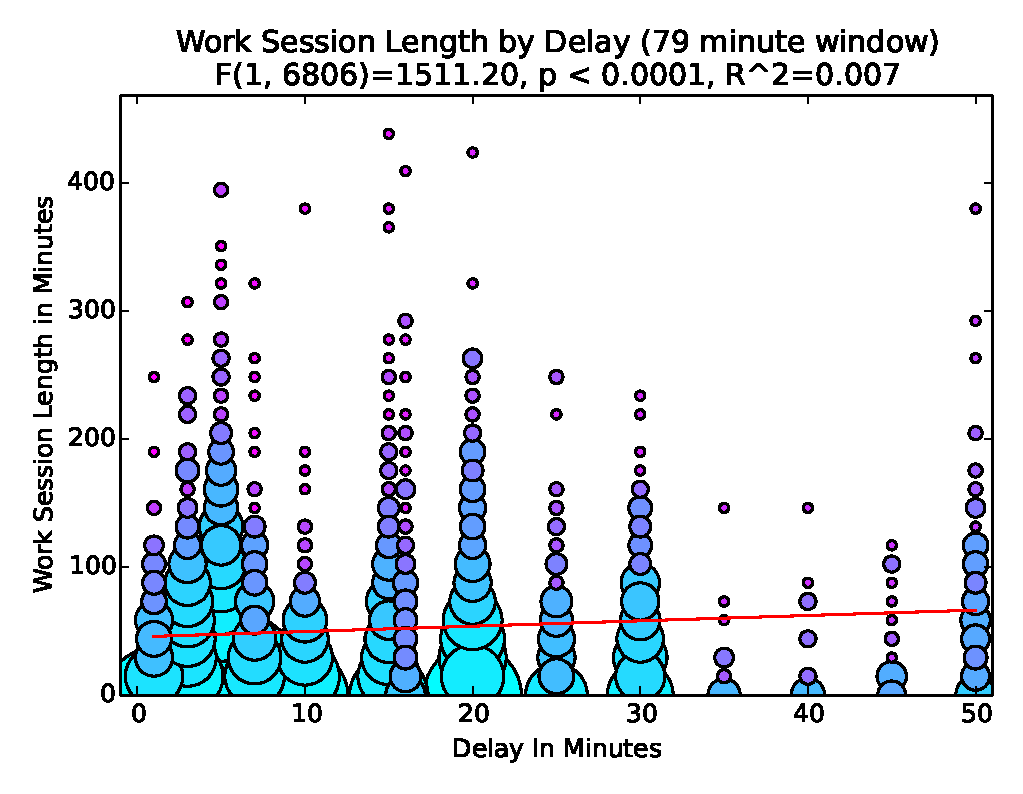
\includegraphics[width=3.3in]{graphs/Work_Session_Length_by_Delay_(79_minute_window).eps}
\caption{Plots the work session length against the feedback delay time. There
  is a slight, nevertheless, statistically significant positive correlation
  between the two.}
\locallabel{fig:session_duration}
\end{figure}

\begin{figure}[!t]
\centering 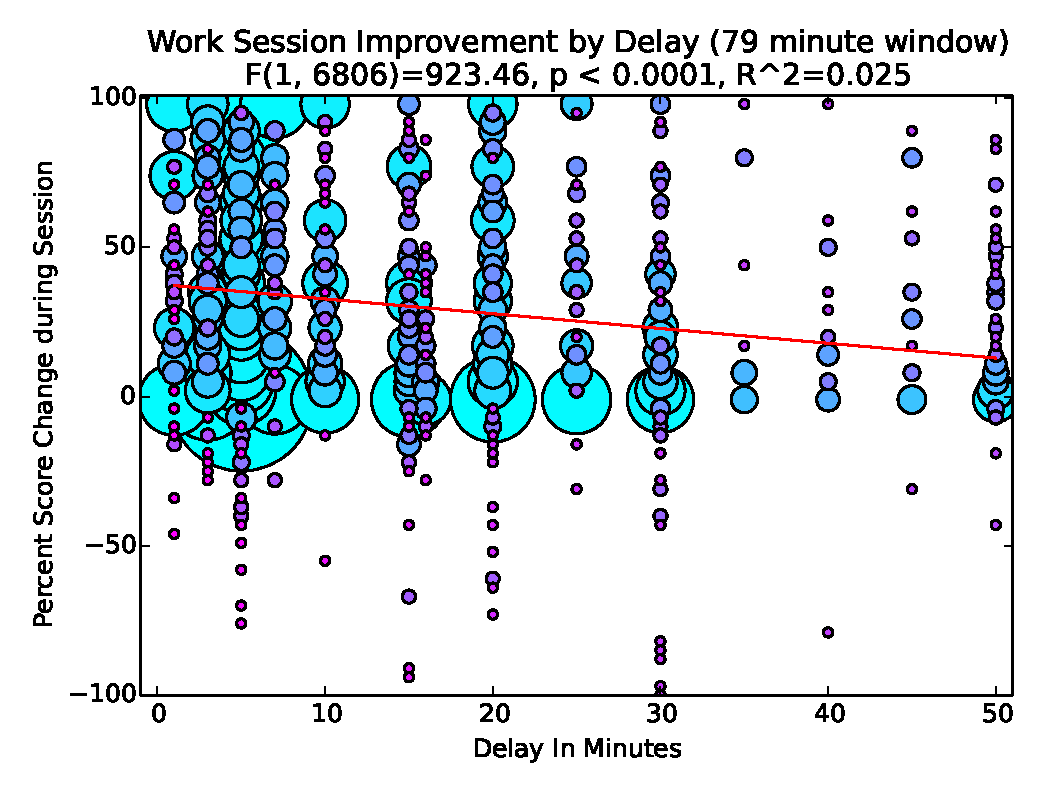
\includegraphics[width=3.3in]{graphs/Work_Session_Improvement_by_Delay_(79_minute_window).eps}
\caption{Plots the improvement in work session grouped by the assignment's
  delay. There is a statistically significant negative correlation between the
  two.}
\locallabel{fig:delay_improvement}
\end{figure}

Finally we consider the impact of the feedback delay on work sessions. We first
consider the effect a change in duration has on the length of a work
session. Figure~\localref{fig:session_duration} shows that there is a
statistically significant, though slight, positive correlation between the
feedback delay and work session length with a seventy-nine minute window
size. The correlation is more prominent with the larger window sizes as
indicated by the red lines in Figure~\localref{fig:window_size}. While we
observe a slight increase in work session length, we cannot absolutely
attribute this to the delay as assignments with delays over thirty minutes were
only given in the latter half of a course. It is common for these assignments
to be more difficult than the initial assignments, and as a result require more
time to complete.

Finally, we look at the impact of the delay on improvement between the first
submission in a work session and the last submission in a work session when
grouped by the feedback delay value. Figure~\localref{fig:delay_improvement}
shows that there is a statistically significant negative correlation between
work session improvement and the feedback delay. While this result may seem
puzzling at first, it is logical. With a smaller delay, groups have more
opportunities to receive feedback and therefore more significantly improve
their work within a single work session. Thus, while their between submission
efficiency may be lower, the net result is increased improvement in the work
session. Conversely, with fewer opportunities for feedback, groups working on
assignments with longer delays have higher efficiency between submissions, but
the relative amount of improvement between work sessions is not as significant.
